\chapter{Mission: MechE}

\emph{\emph{MechE} is a RECON+ mission grabbing prototype data from
  the Mechanical Engineering Laboratory.}

\section{Play Area}
\vspace{-2\parskip}
\noindent\begin{stdminipage}{\linewidth-(3in+1.5em)}
\vspace{0pt}   
\noindent
The Deployment Zones extend~4'' out along the full extent of the long
play area edges.

A Network Terminal is placed at the play area center.

Place four Tech-Coffins, each equipped with a Datacube, along the long
centerline of the play area, two~6'' from the short edges and two~12''
from the short edges.

\section{Mission Rules}

The following short skills and equipment are available:

\end{stdminipage}
\hfill
\begin{minipage}[t]{3in}\centering
\vspace{4pt}   
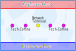
\includegraphics{maps/map-mech}
\end{minipage}

{\setlength\fboxrule{2pt}
\cfbox{LimeGreen}{\begin{minipage}{6.5in}
  \colorbox{LimeGreen}{\parbox{\linewidth-2\fboxsep}{\textcolor{White}{\textbf{\large Smash Tech-Coffin} \hfill Short Skill}}}\\
  \colorbox{SkyBlue}{\parbox{\linewidth-2\fboxsep}{\textcolor{White}{Attack}}}

  \medskip
  \textsc{Requirements}
  \begin{squishitemize}
  \item The user must be a Specialist Troop model (not a marker) in
    base contact with a Tech-Coffin equipped with a Datacube.

%  \item The user must not already be equipped with a Datacube, or, if
%    it also possesses Baggage equipment, must not be equipped with two
%    Datacubes.
  \end{squishitemize}

  \medskip
  \colorbox{Gray!24}{\begin{minipage}{\linewidth-2\fboxsep}

  \medskip      
      \textsc{Effects}
      \begin{squishitemize}
%      \item Allows the user to make a Normal WIP roll to break the
%        Tech-Coffin's protections and extract the Datacube.  Hackers
%        receive a +3 MOD.

      \item The user makes a Normal WIP roll to extract the Datacube.

      \item If passed, the Tech-Coffin unequips a Datacube and
        the user equips it. % (or an additional
        %Datacube if it possesses Baggage and was already equipped with
        %one).
        
%      \item This skill may be invoked as many times as desired if the
%        user continues to fail.
      \end{squishitemize}
    \end{minipage}}
\end{minipage}}}

{\setlength\fboxrule{2pt}
\cfbox{LimeGreen}{\begin{minipage}{6.5in}
  \colorbox{LimeGreen}{\parbox{\linewidth-2\fboxsep}{\textcolor{White}{\textbf{\large Grab Datacube} \hfill Short Skill}}}\\
  \colorbox{SkyBlue}{\parbox{\linewidth-2\fboxsep}{\textcolor{White}{Attack}}}

  \medskip
  \textsc{Requirements}
  \begin{squishitemize}
  \item The user must be a model (not a marker) in base contact with a
    a Datacube marker or a friendly troop equipped with a Datacube.
    Note that the user does NOT have to be a Specialist Troop to
    execute this skill.

%  \item The user must not already be equipped with a Datacube, or, if
%    it also possesses Baggage equipment, must not be equipped with two
%    Datacubes.
  \end{squishitemize}

  \medskip
  \colorbox{Gray!24}{\begin{minipage}{\linewidth-2\fboxsep}

      \medskip
      \textsc{Effects}
      \begin{squishitemize}
      \item The user designates a Datacube marker or a friendly model
        equipped with a Datacube in base contact from which to grab a
        Datacube.
        
%      \item The user automatically equips a Datacube (or an additional
%        Datacube if it possesses Baggage and was already equipped with
%        one).
   
      \item If a friendly troop was designated, it unequips a
        Datacube.  If a Datacube marker was designated, it is removed
        from play.

      \item The user automatically equips the Datacube.
      \end{squishitemize}
  \end{minipage}}
\end{minipage}}}

{\setlength\fboxrule{2pt}
\cfbox{LimeGreen}{\begin{minipage}{6.5in}
  \colorbox{LimeGreen}{\parbox{\linewidth-2\fboxsep}{\textcolor{White}{\textbf{\large Drop Datacube} \hfill Short Skill, ARO}}}\\
  \colorbox{SkyBlue}{\parbox{\linewidth-2\fboxsep}{\textcolor{White}{Attack}}}

  \medskip
  \textsc{Requirements}
  \begin{squishitemize}
  \item The user must be equipped with a Datacube.
  \end{squishitemize}

  \medskip
  \colorbox{Gray!24}{\begin{minipage}{\linewidth-2\fboxsep}

      \medskip
      \textsc{Effects}
      \begin{squishitemize}
%      \item By spending a short skill or ARO, the user automatically
%        unequips one Datacube.  Its player places a Datacube marker in
%        base contact with the model or at any point in its movement if
%        it made any.
      \item The user automatically unequips one Datacube.  Place a
        Datacube marker in base contact or at any point in the model's
        movement.
      \end{squishitemize}
  \end{minipage}}
\end{minipage}}}

{\setlength\fboxrule{2pt}
\cfbox{Black}{\begin{minipage}{6.5in}
  \colorbox{Black}{\parbox{\linewidth-2\fboxsep}{\textcolor{White}{\textbf{\large Datacube} \hfill Automatic Equipment}}}\\
  \colorbox{White}{\parbox{\linewidth-2\fboxsep}{Obligatory}}

  \medskip
  \textsc{Requirements}
  \begin{squishitemize}
  \item A model cannot ever be equipped with more than one Datacube,
    unless it also possesses Baggage equipment, in which case it may
    equip two.
  \end{squishitemize}
  
  \medskip
  \colorbox{Gray!24}{\begin{minipage}{\linewidth-2\fboxsep}

      \medskip
      \textsc{Effects}
      \begin{squishitemize}
%      \item No model may ever be equipped with more than one Datacube,
%        unless it also possesses Baggage equipment, in which case it
%        may be equipped with two Datacubes.
        
      \item Immediately upon the user entering a Null state (e.g.,
        going Unconscious), their model being replaced with a marker
        (e.g., returning to the Camouflaged state), or being removed
        from the game (e.g., becoming Dead), they unequip the Datacube
        and a Datacube marker is placed by their player in base
        contact with the user or its former position.

        %If they possessed multiple Datacubes, a Datacube marker is
        %placed for each.
      \end{squishitemize}
  \end{minipage}}
\end{minipage}}}

\section{Scoring}

Players may score up to~10 objective points via the following
conditions at game end:
\begin{squishitemize}  
\item 1pt for any model having equipped a Datacube at any point in the game.
\item 1pt for each Datacube equipped by any model of yours.
\item 2pt if you have a model equipped with a Datacube in your Deployment Zone.
\item 2pts if your Special Agent is equipped with a Datacube.
%\item 1pt if the opposing Special Agent is in a Null state or eliminated.
\item 1pt if more points of the opposing army list have been destroyed.
\end{squishitemize}

\vfill
\vbox to 0pt{}